\documentclass[a4paper,12pt]{article}
\usepackage[top=2cm,right=2cm,bottom=2cm,left=2cm]{geometry}
\usepackage[portuguese]{babel}
\usepackage[utf8]{inputenc}
\usepackage[T1]{fontenc}
\usepackage{amsfonts,amsmath,amssymb}
\usepackage{siunitx}
\usepackage{hyperref}
\usepackage{graphicx}
%\usepackage{xwatermark}
\usepackage{xcolor}
\usepackage{import}
%\newwatermark[allpages,scale=6,color=red!15,angle=60,xpos=-60pt,ypos=30pt]{FA470}

\newcommand{\chapternumber}[1]{\textbf{Capítulo #1}}
\newcommand{\chaptertitle}[1]{\uppercase{\textbf{#1}}}

\begin{document}  
	\import{sections/}{header}
	
	\begin{enumerate}
		\item Uma mola de rigidez $k=\SI{500}{\newton/\meter}$ está montada contra o bloco de \SI{10}{\kilogram}. Se o bloco está sujeito à força $F=\SI{500}{\newton}$, determine a sua velocidade em $s=\SI{0.5}{\meter}$. Quando $s=0$, o bloco está em repouso e a mola está descomprimida. A superfície de contato é lisa.
		
		$\textbf{\text{Resposta}}\Rightarrow v=\SI{5.24}{\meter/\second}$
		
		\begin{center}
			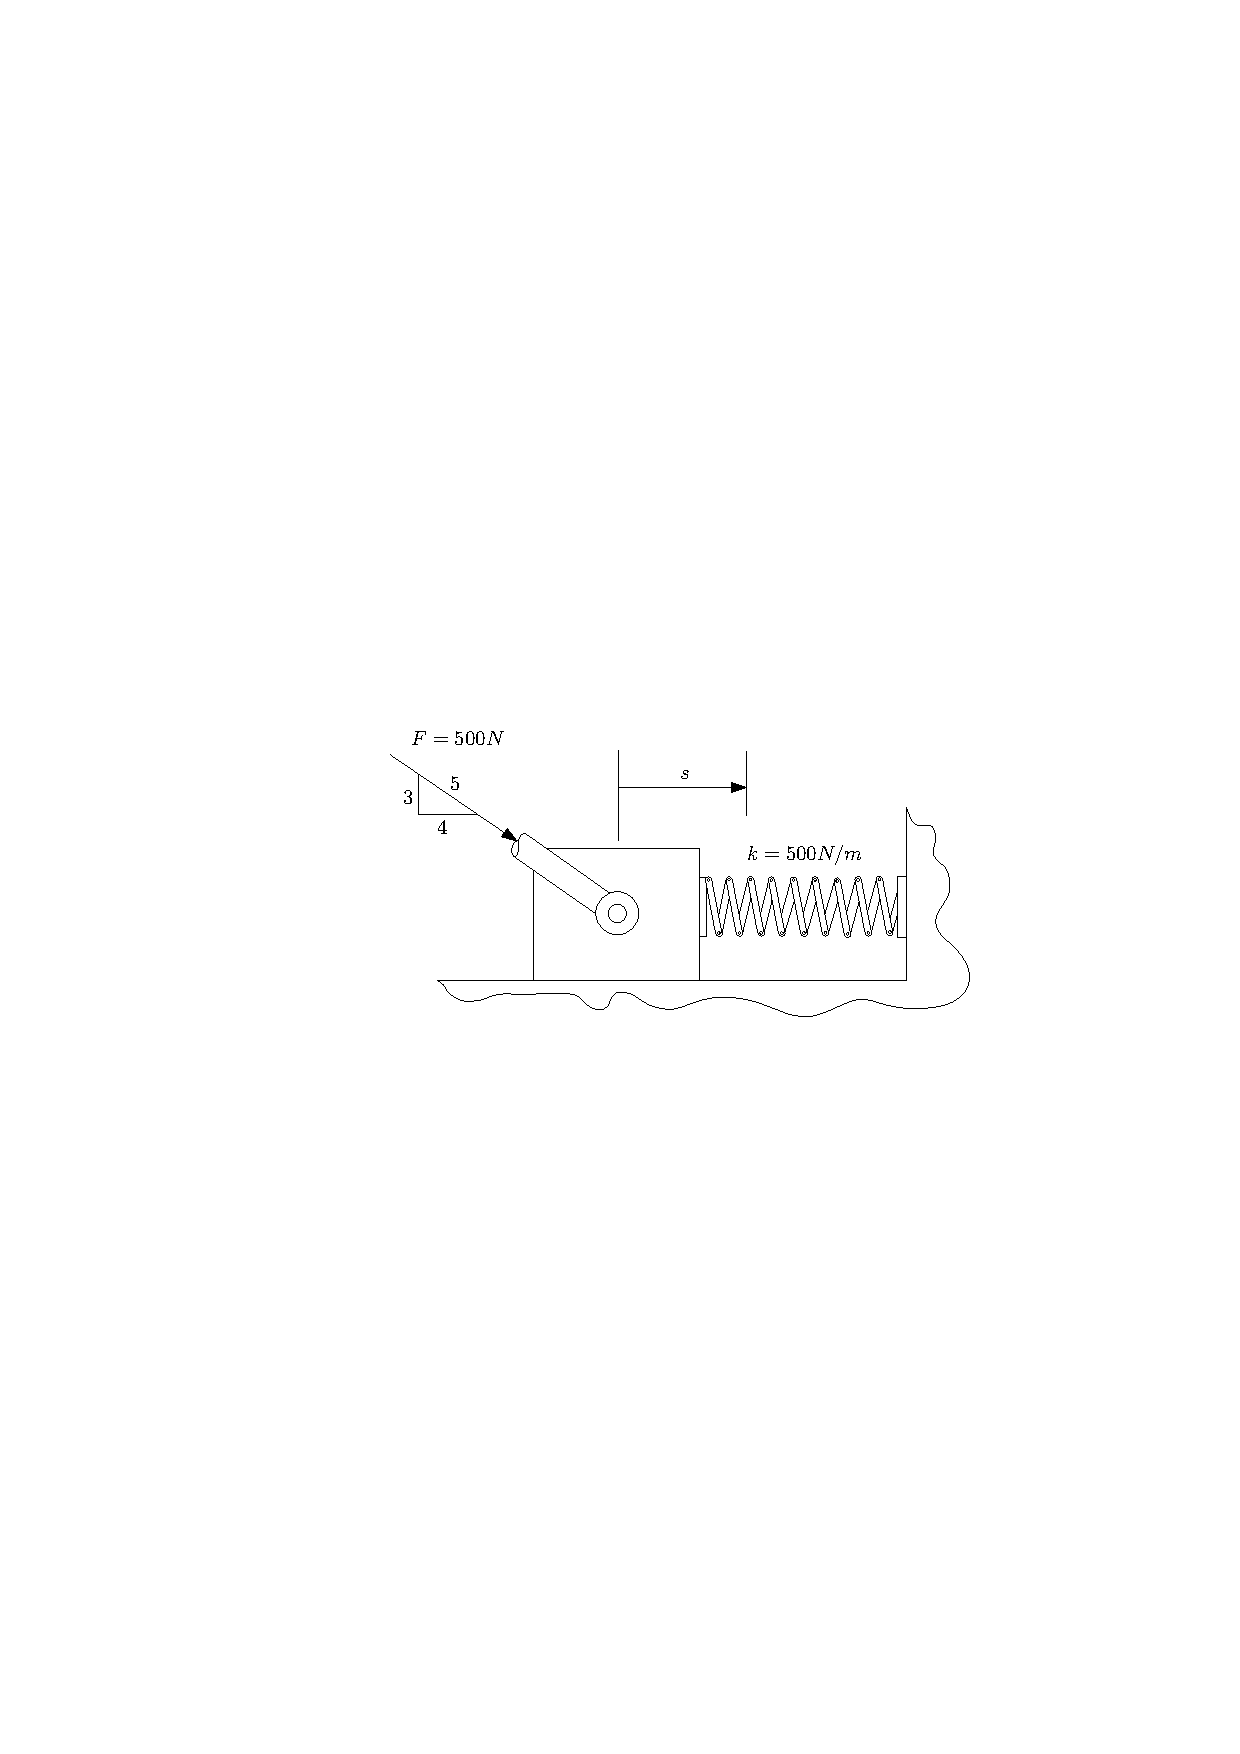
\includegraphics[scale=1.2]{images/draw_1.pdf}
		\end{center}
		
		\item Se o bloco $A$ de \SI{5}{\kilogram} escorrega para baixo no plano inclinado com uma velocidade constante quando $\theta=\SI{30}{^{\circ}}$, determine a aceleração do bloco quando $\theta=\SI{45}{^{\circ}}$
		
		$\textbf{\text{Resposta}}\Rightarrow a=\SI{2.9318}{\meter/\second^{2}}$
		
		\vspace{1.5cm}
		\begin{flushright}
			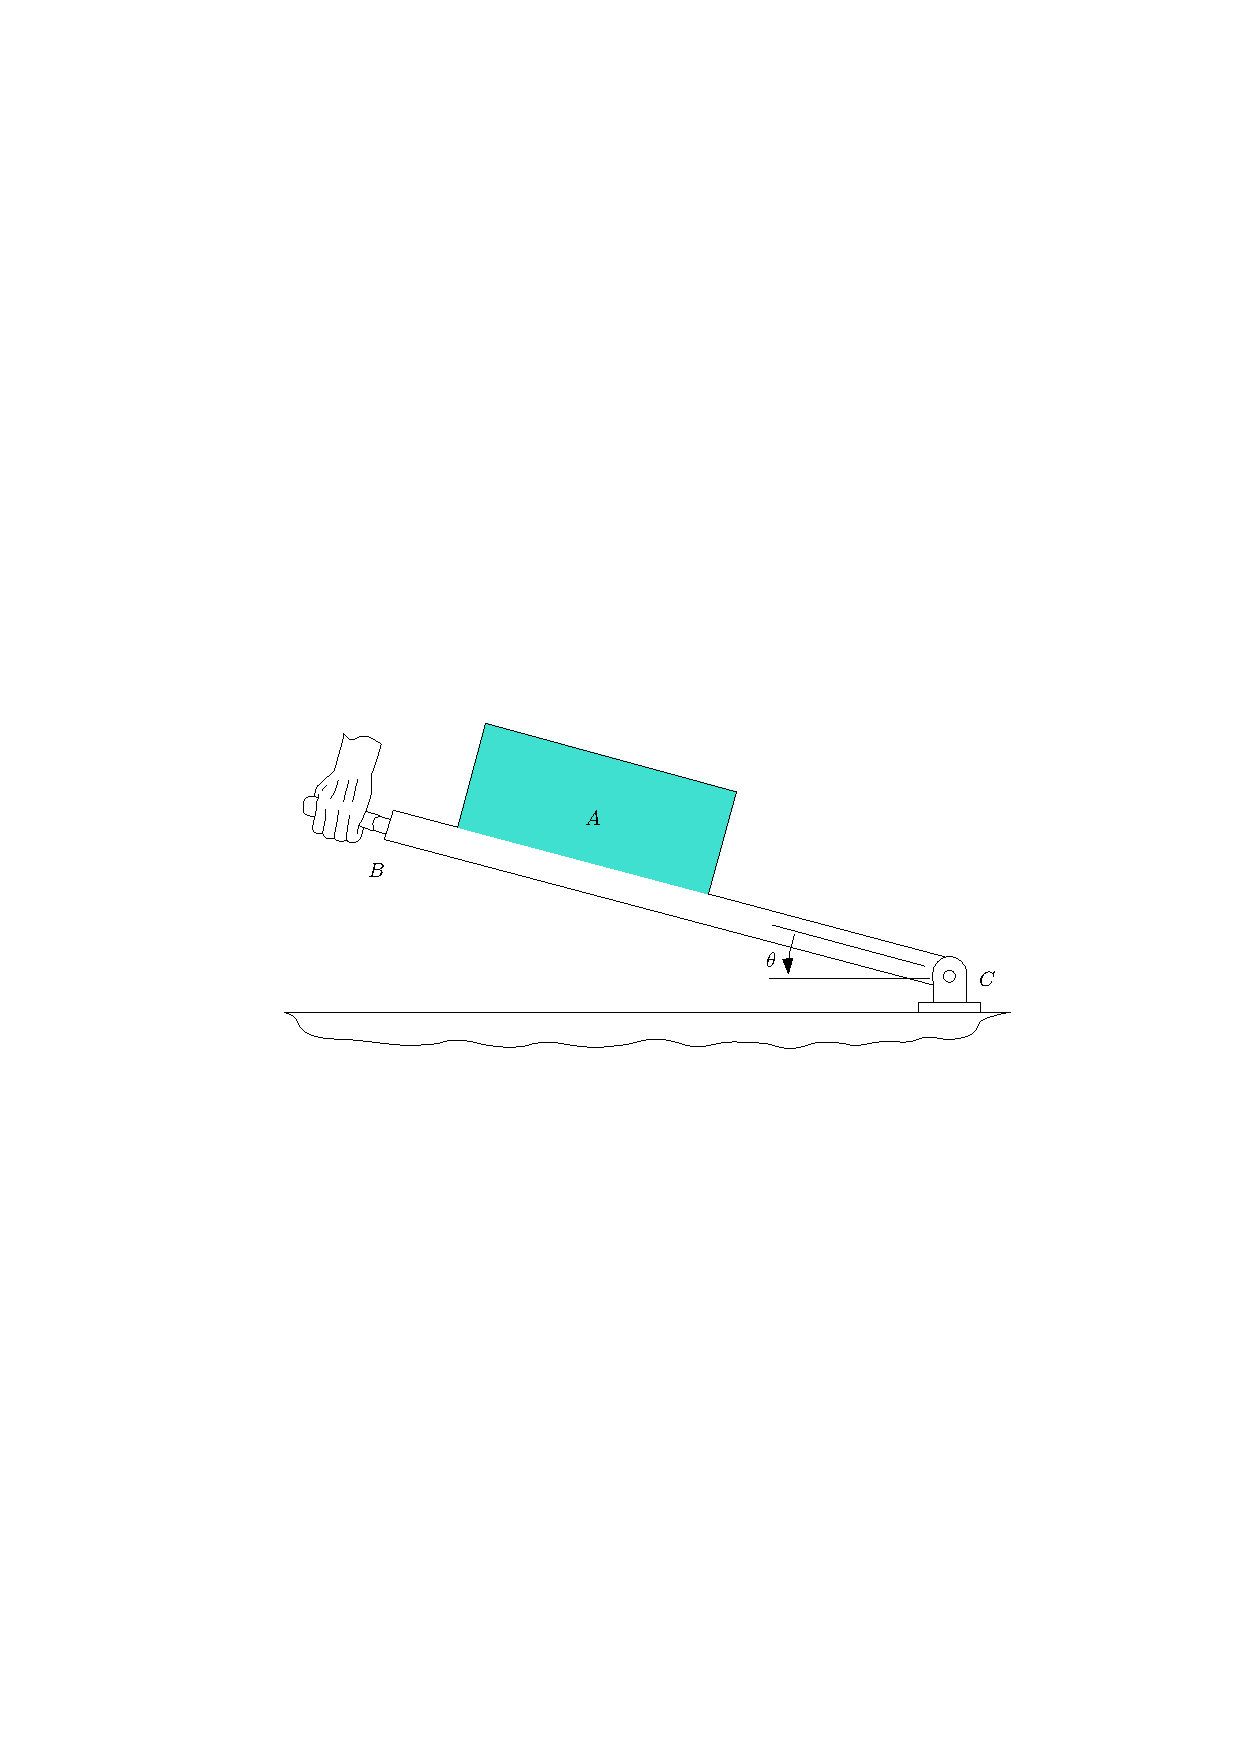
\includegraphics[scale=1]{images/draw_2.pdf}
		\end{flushright}
		
		\newpage
		\item O anel $C$ de $\SI{1}{\kilogram}$ ajusta-se livremente no eixo liso. Se a mola está livre quando $s=0$ e ao anel é dada uma velocidade de $\SI{4.5}{\meter/\second}$, determine a velocidade do anel quando $s=\SI{0.3}{\meter}$
		
		$\textbf{\text{Resposta}}\Rightarrow v=\SI{4.445}{\meter/\second}$
		
		\vspace{-1cm}
		\begin{flushright}
			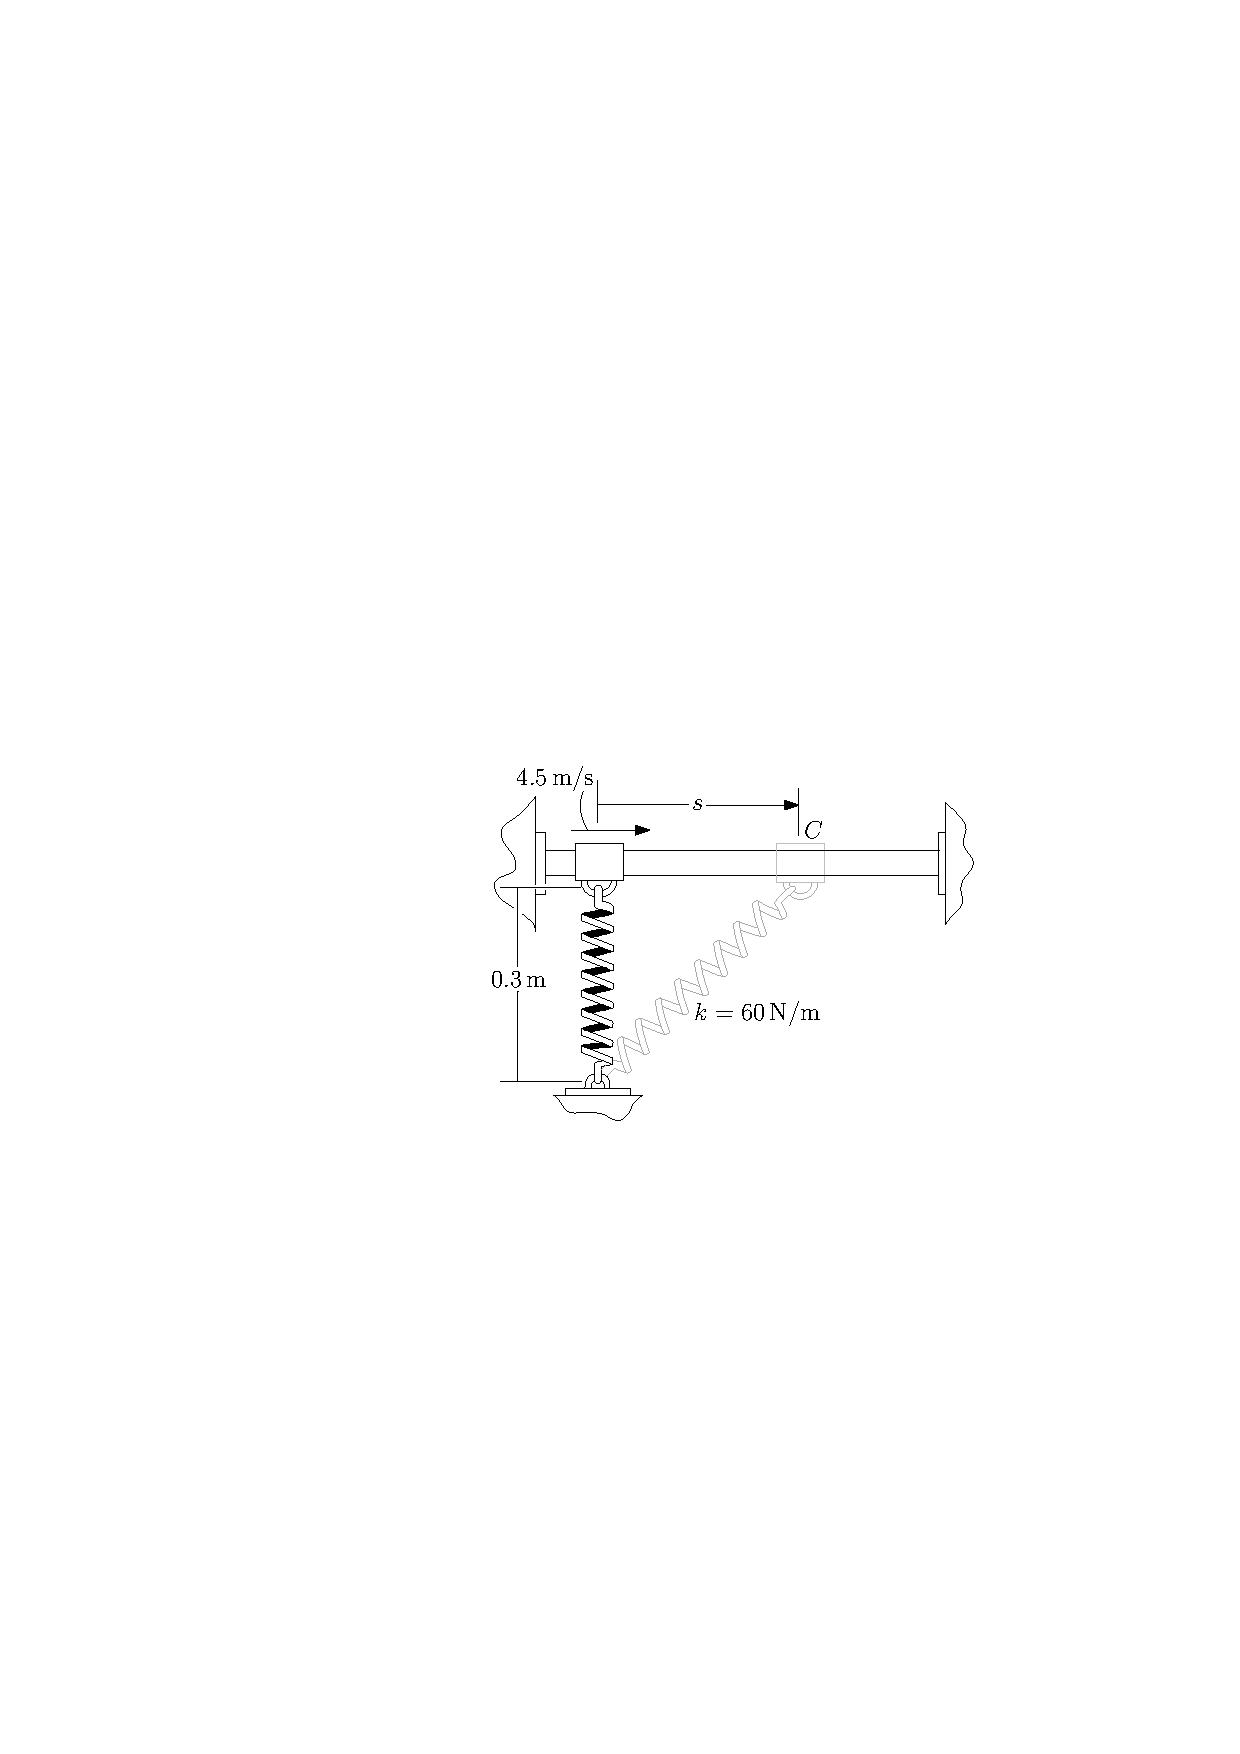
\includegraphics[scale=1.2]{images/draw_14.pdf}
		\end{flushright}
		
		\item A caixa tem massa de \SI{80}{\kilogram} e está sendo puxada por uma corrente que está sempre direcionada a $\SI{20}{^{\circ}}$ da horizontal, como mostrado. Determine a aceleração da caixa em $t=\SI{2}{\second}$ se o coeficiente de atrito estático é $\mu_{s}=0.4$, o coeficiente de atrito cinético é $\mu_{k}=0.3$, e a força de reboque é $P=(90\,t^{2})$, onde $t$ é dado em, segundos
		
		$\textbf{\text{Resposta}}\Rightarrow a=\SI{1.75}{\meter/\second^{2}}$
		
		\vspace{-1cm}
		\begin{flushright}
			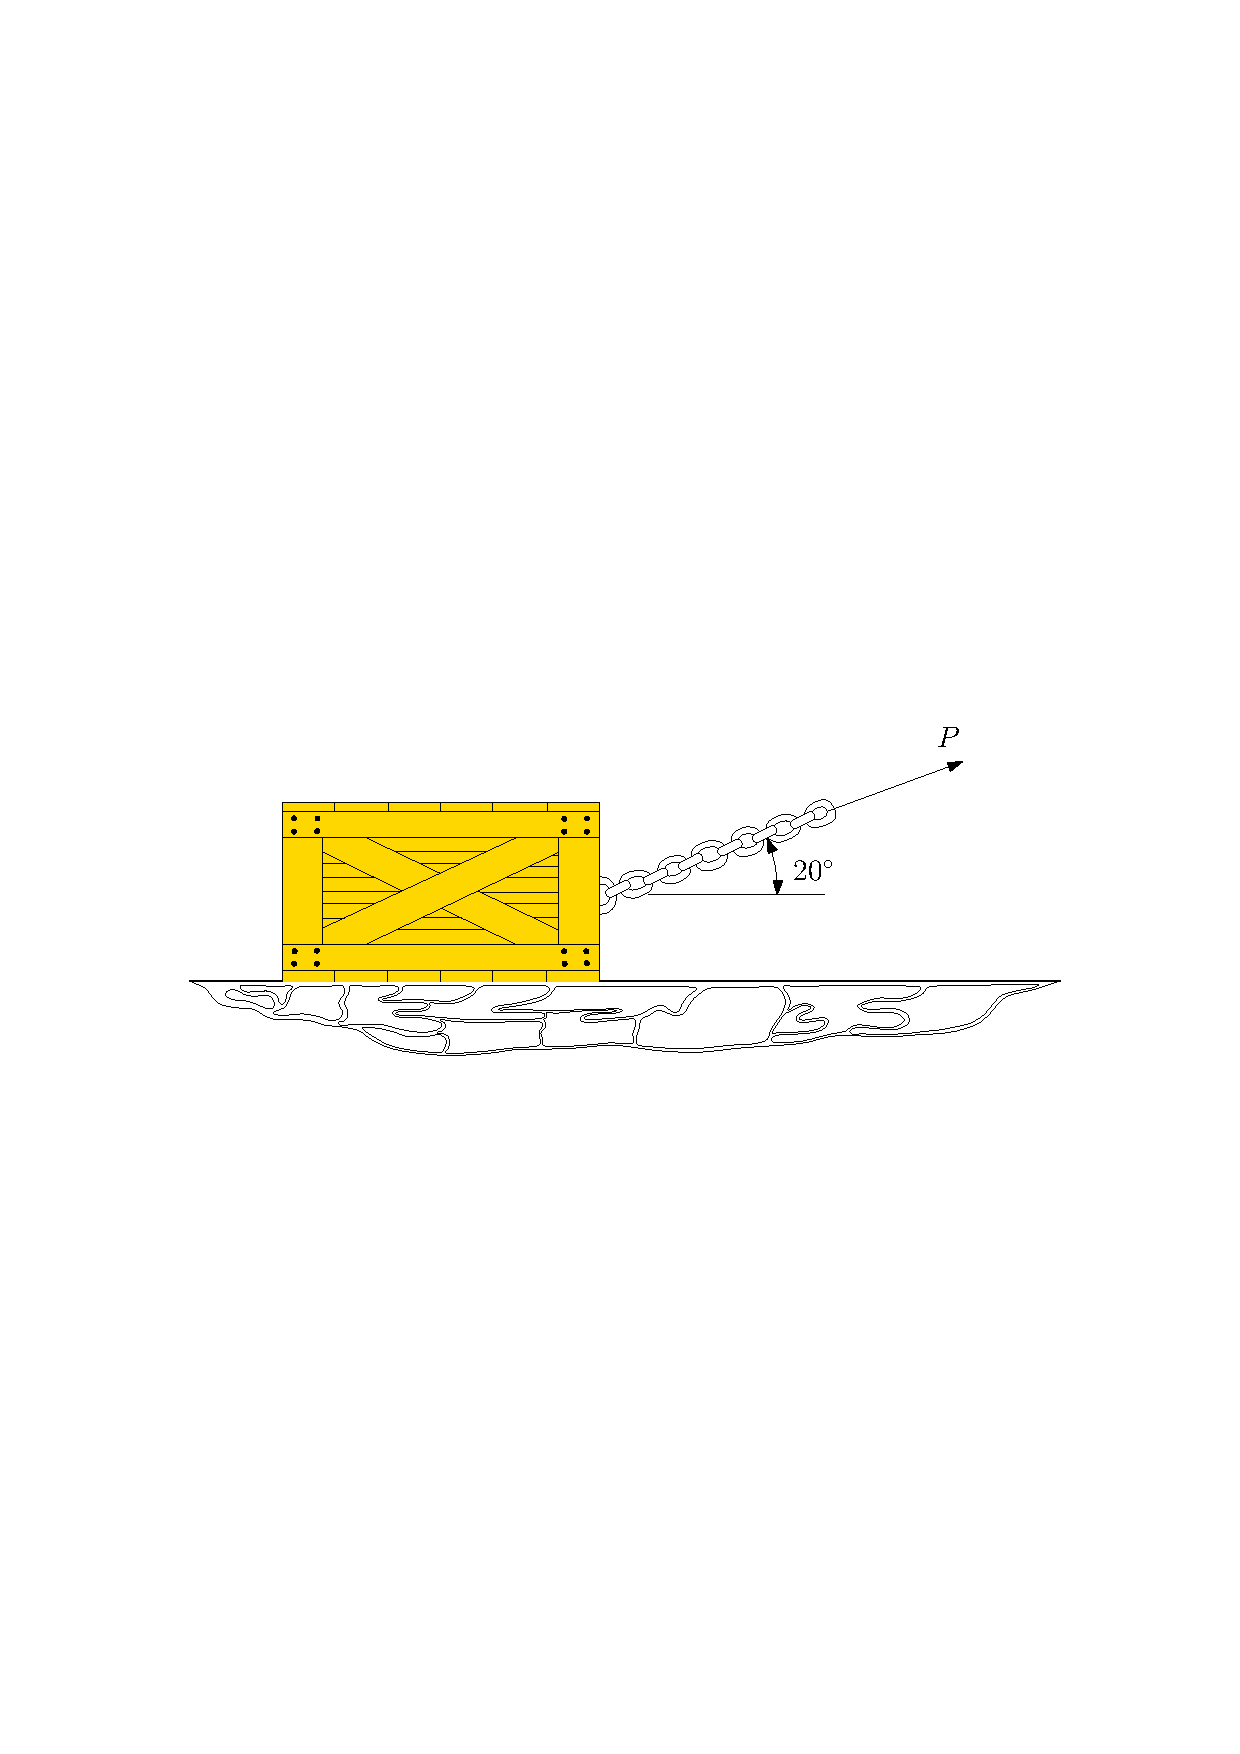
\includegraphics[scale=.9]{images/draw_3.pdf}
		\end{flushright}
		
		\item O carro de corrida tipo \textit{dragster} de \SI{600}{\kilogram} está se movendo com velocidade de \SI{125}{\meter/\second} quando o motor é desligado e o paraquedas de freio é aberto. Se a resistência do ar imposta sobro o \textit{dragster} devido ao paraquedas é $F_{D}=(6000+0.9\,v^{2})\,\SI{}{N}$, onde $v$ é dado em \SI{}{\meter/\second}, determine o tempo necessário para o \textit{dragster} chegar ao repouso. 
		
		$\textbf{\text{Resposta}}\Rightarrow t=\SI{8.10}{\second}$
		
		\begin{flushright}
			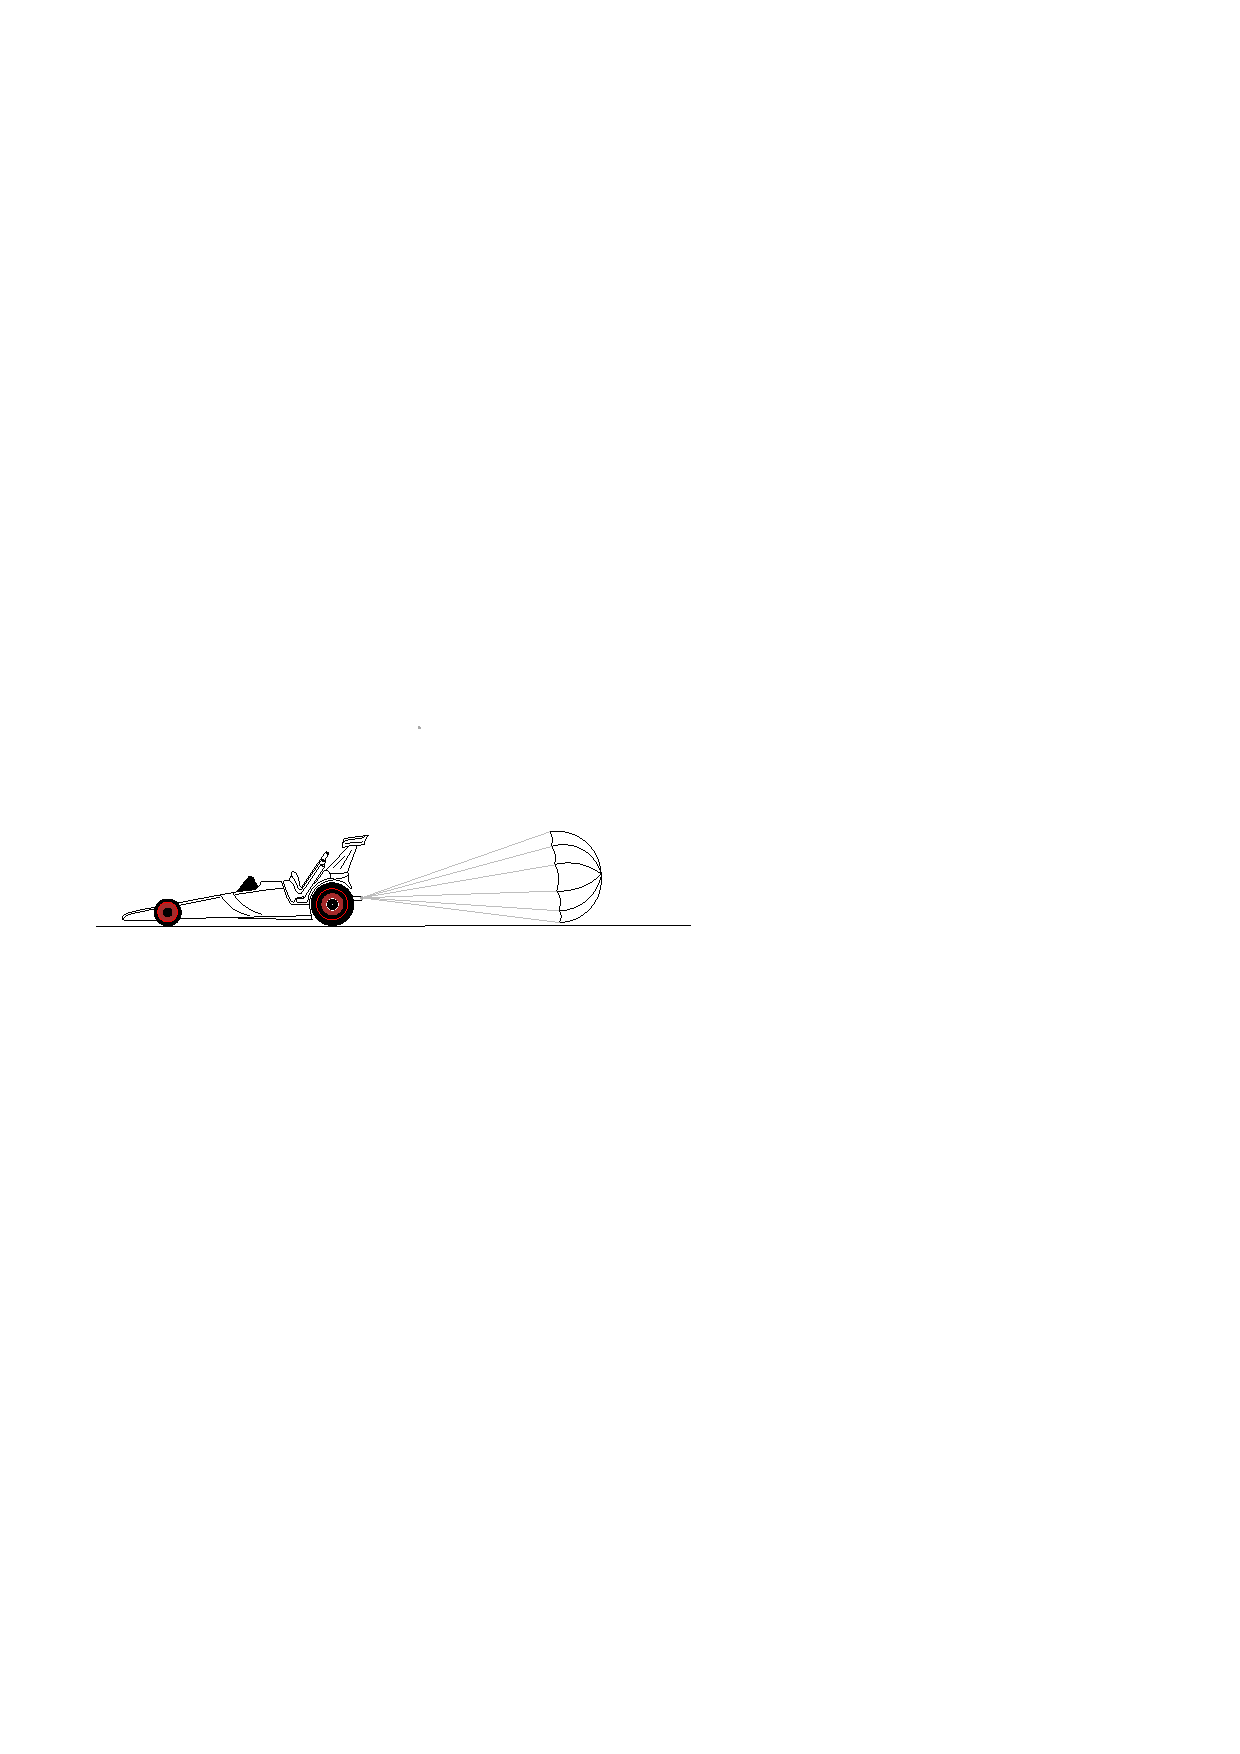
\includegraphics[scale=1.3]{images/draw_5.pdf}
		\end{flushright}
		
		\newpage
		\item Determine a velocidade máxima que o jipe pode se mover sobre o cume do monte sem perder o contato com a estrada.
		
		$\textbf{\text{Resposta}}\Rightarrow v=\SI{27.12}{\meter/\second}$
		
		\begin{flushright}
			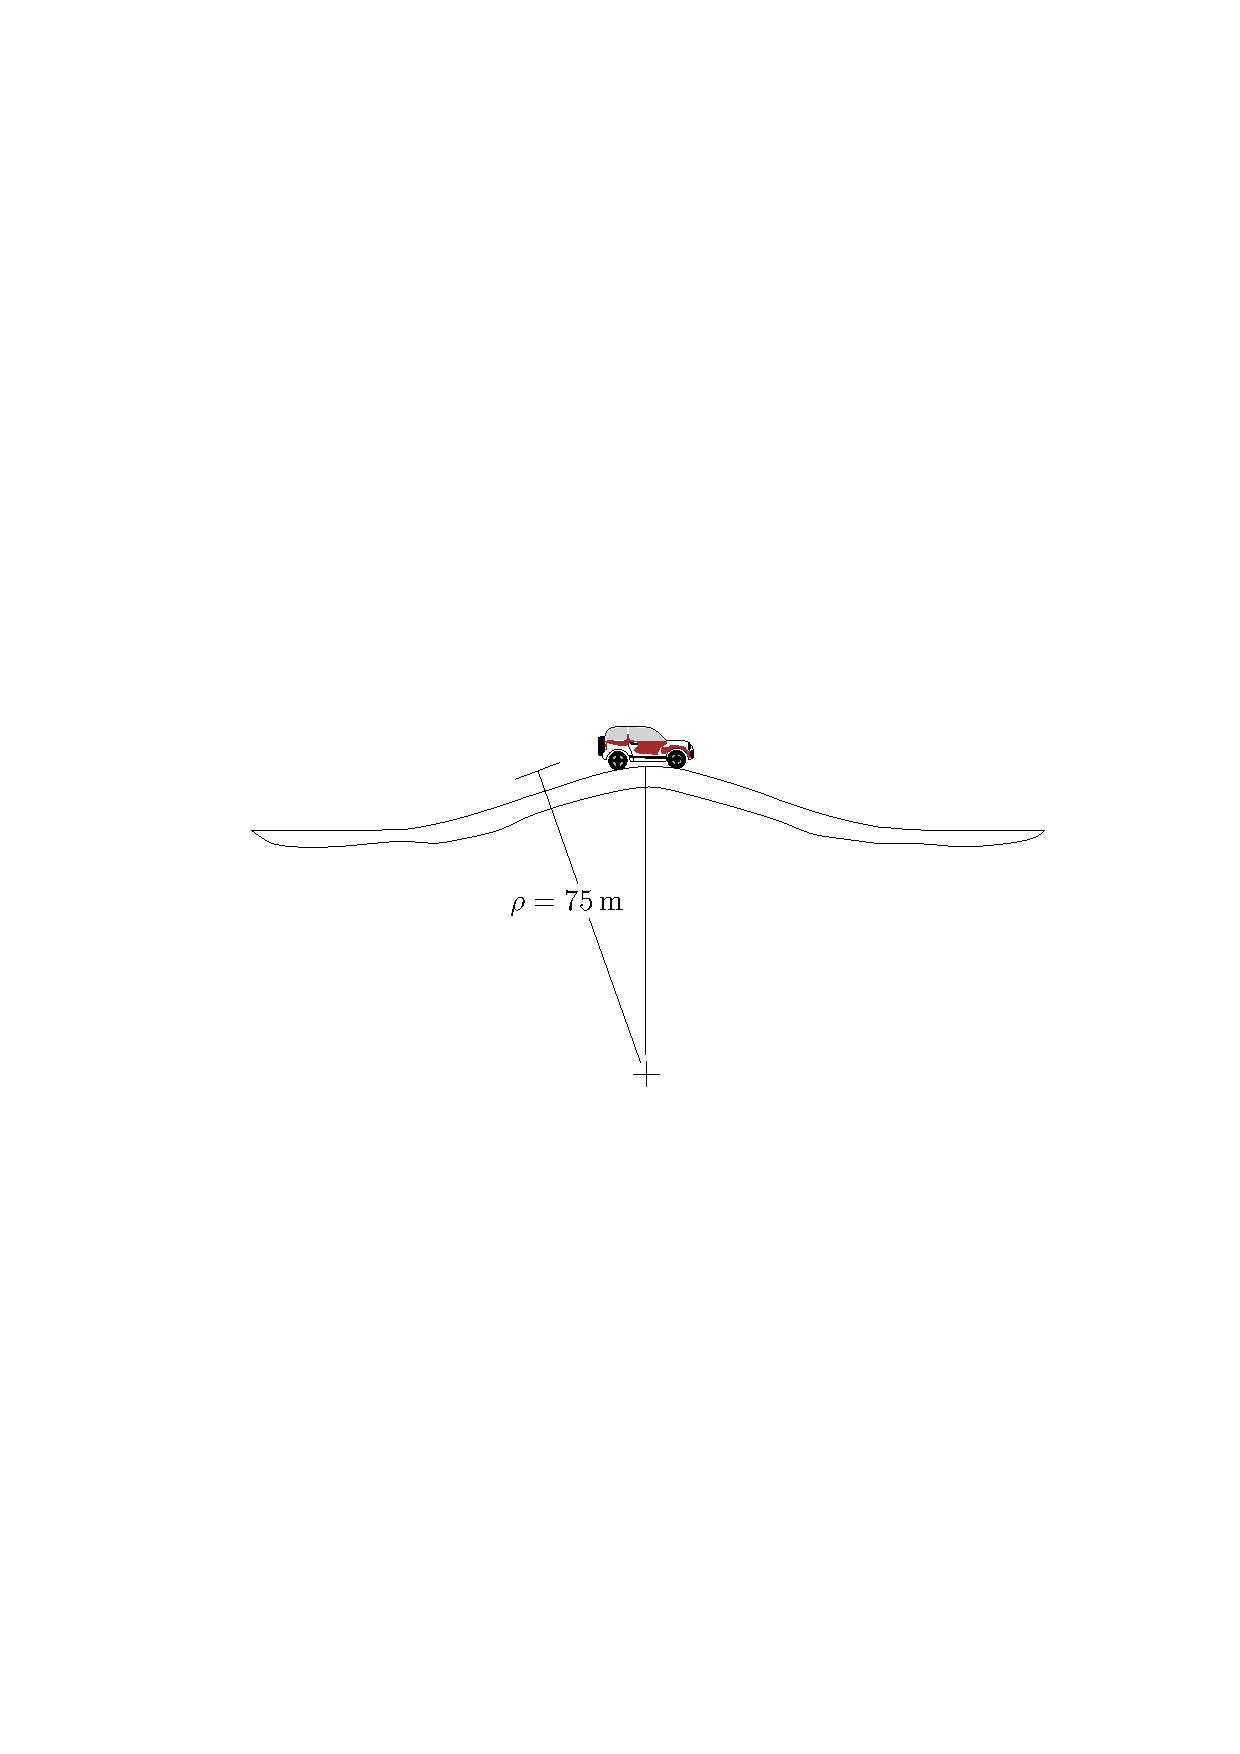
\includegraphics[scale=.8]{images/draw_4.pdf}
		\end{flushright}
		
		\item Um homem tendo massa de \SI{75}{\kilogram} senta na cadeira que está presa por um pino à estrutura $BC$. Se o homem está sempre sentado em um posição vertical, determine as reações horizontal e vertical da cadeira sobre o homem no instante $\theta=\SI{45}{^{\circ}}$. Neste instante ele tem uma velocidade de \SI{6}{\meter/\second} que está acelerando a \SI{0.5}{\meter/\second$^{2}$}
		
		\textbf{Resposta}
		$
		\begin{cases}
		R_{x}=\SI{217}{\newton}\\
		R_{y}=\SI{517}{\newton}
		\end{cases}
		$
		\vspace{-1.4cm}
		\begin{flushright}
			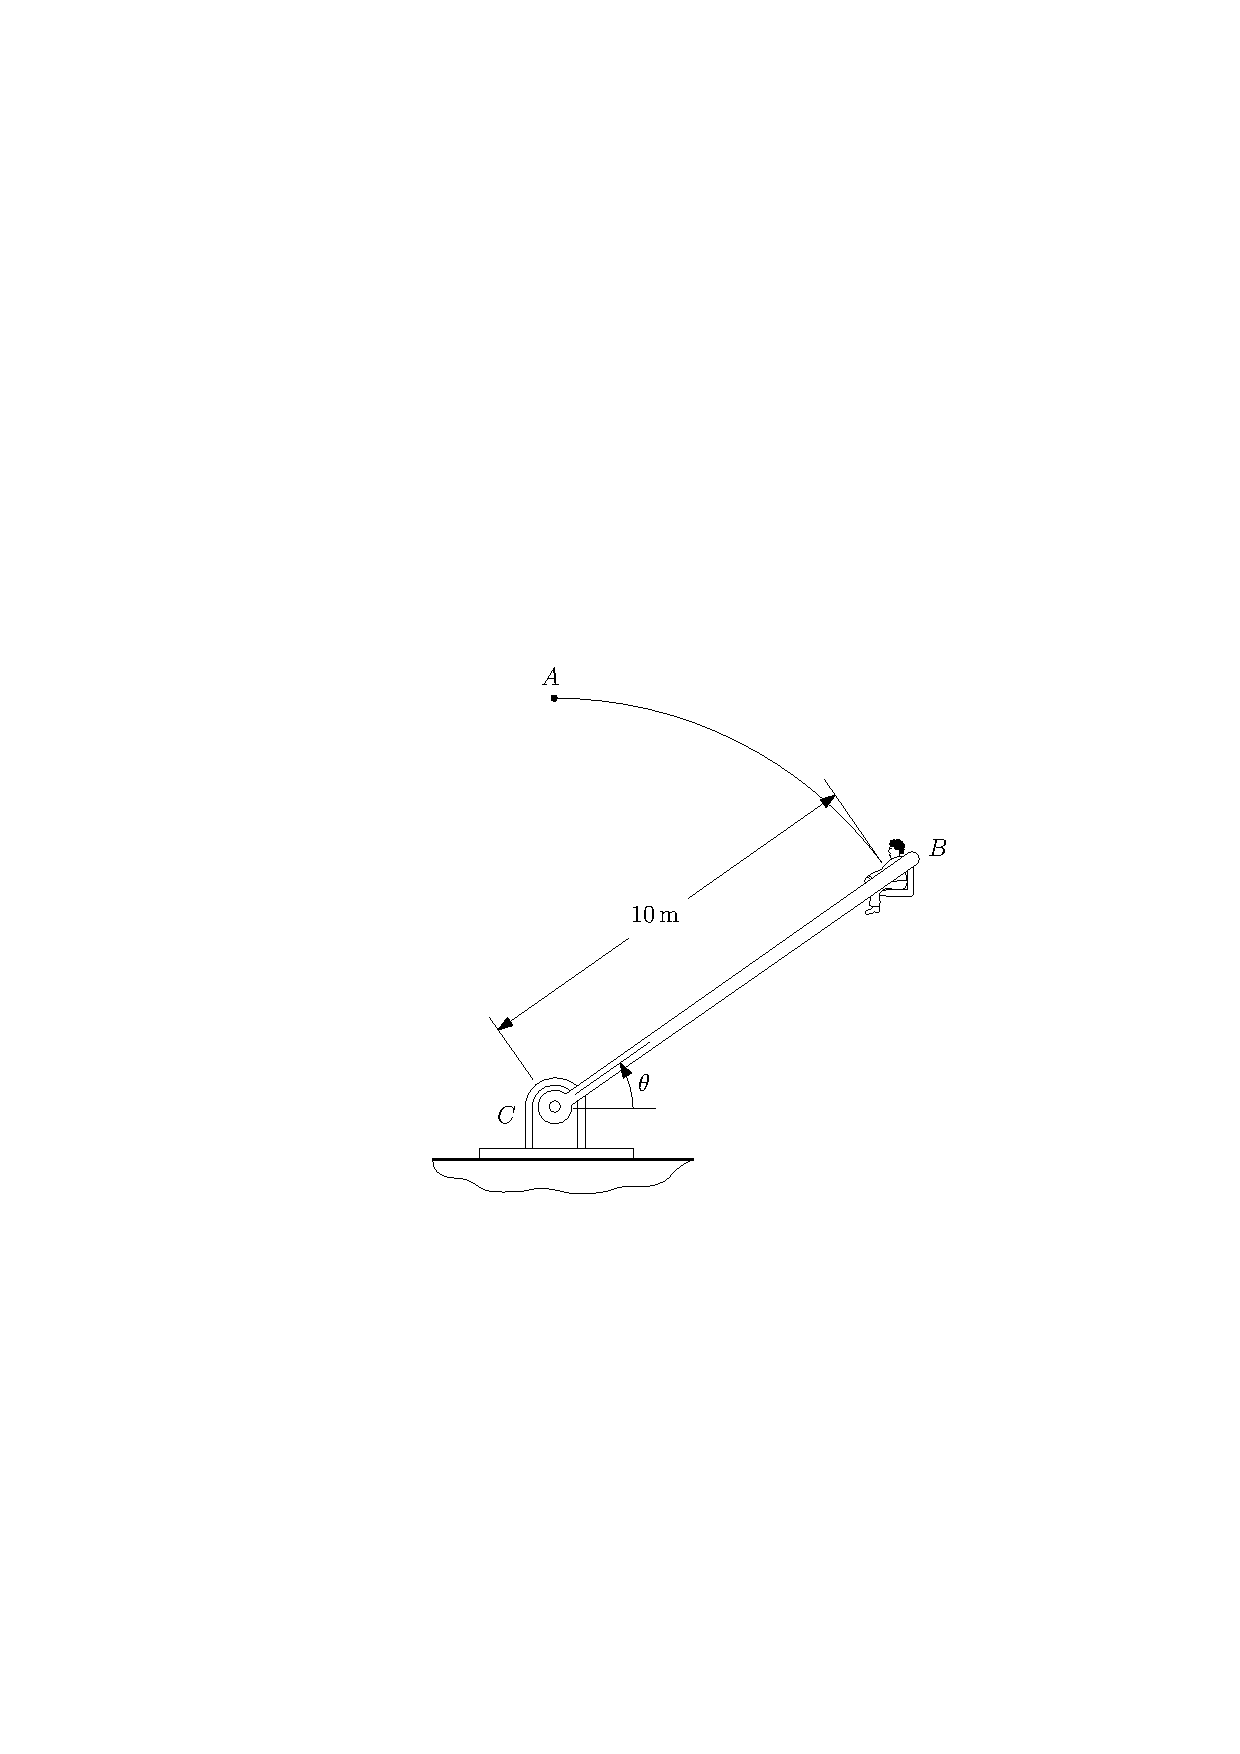
\includegraphics[scale=1]{images/draw_11.pdf}
		\end{flushright}
		
		\item Um acrobata tem peso de \SI{750}{\newton} ($m\approx\SI{75}{\kilogram}$) e está sentado em uma cadeira que está fixada no topo de um mastro, como mostrado. Se por um acionamento mecânico o mastro gira para baixo com uma razão constante a partir de $\theta=\SI{0}{^{\circ}}$ de tal maneira que o centro de massa $G$ do acrobata mantenha uma velocidade constante $v=\SI{3}{\meter/\second}$, determine o ângulo $\theta$ no qual ele começa a "voar"\,para fora da cadeira. Despreze o atrito e suponha que a distância do axial $O$ a $G$ é $\rho=\SI{4.5}{\meter}$ 
		
		$\textbf{\text{Resposta}}\Rightarrow \theta=\SI{78.2}{^{\circ}}$
		
		\begin{flushright}
			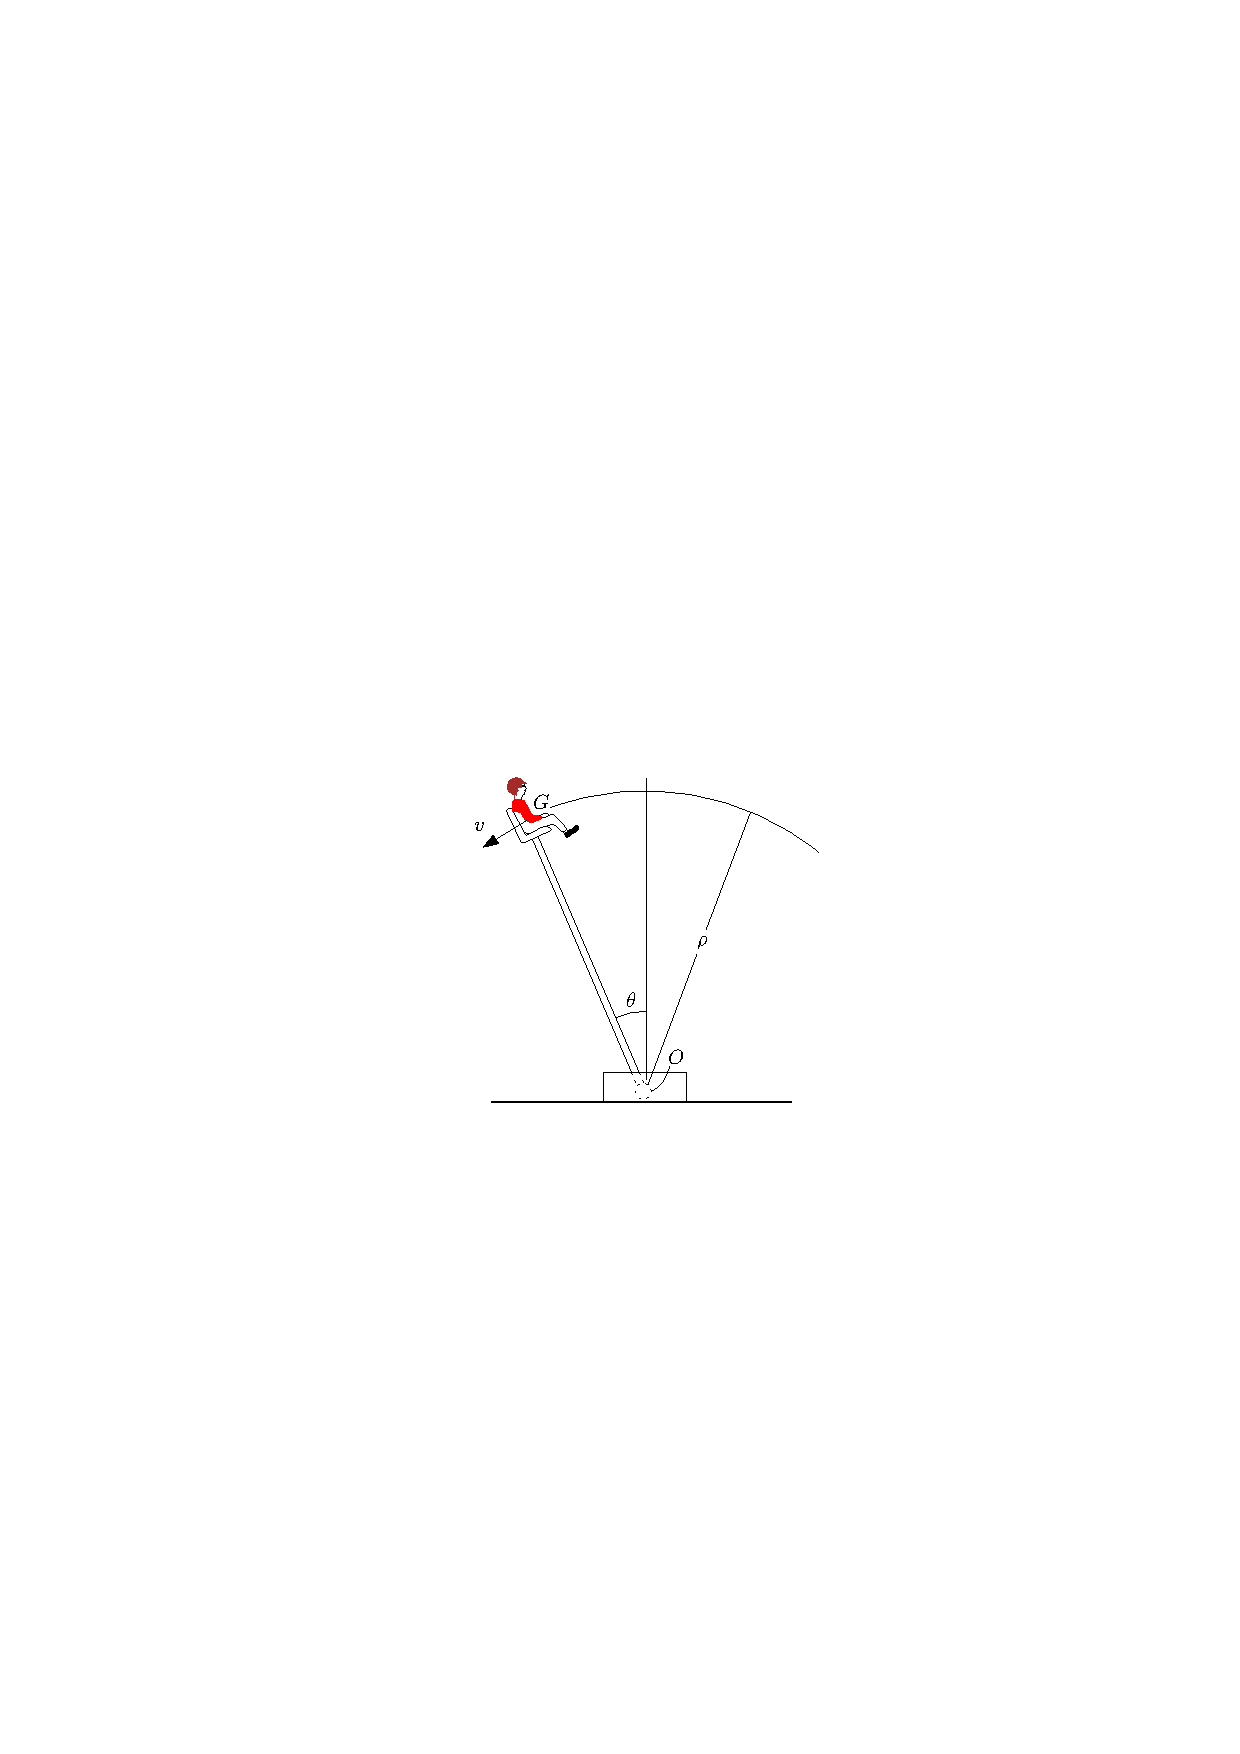
\includegraphics[scale=1.1]{images/draw_9.pdf}
		\end{flushright}
		
		\item Se uma bola tem massa de \SI{30}{\kilogram} e velocidade de $v=\SI{4}{\meter/\second}$ no instante que ela está no ponto mais baixo, $\theta=\SI{0}{^{\circ}}$. Determine a tração na corda e a taxa na qual a velocidade da bola está desacelerando no instante $\theta=\SI{20}{^{\circ}}$. Despreze a dimensão da bola.
		
		\textbf{Resposta}
		$
		\begin{cases}
		T=\SI{361}{\newton}\\
		a_{t}=\SI{3.36}{\meter/\second^{2}}
		\end{cases}
		$
		
		\vspace{-1cm}
		\begin{flushright}
			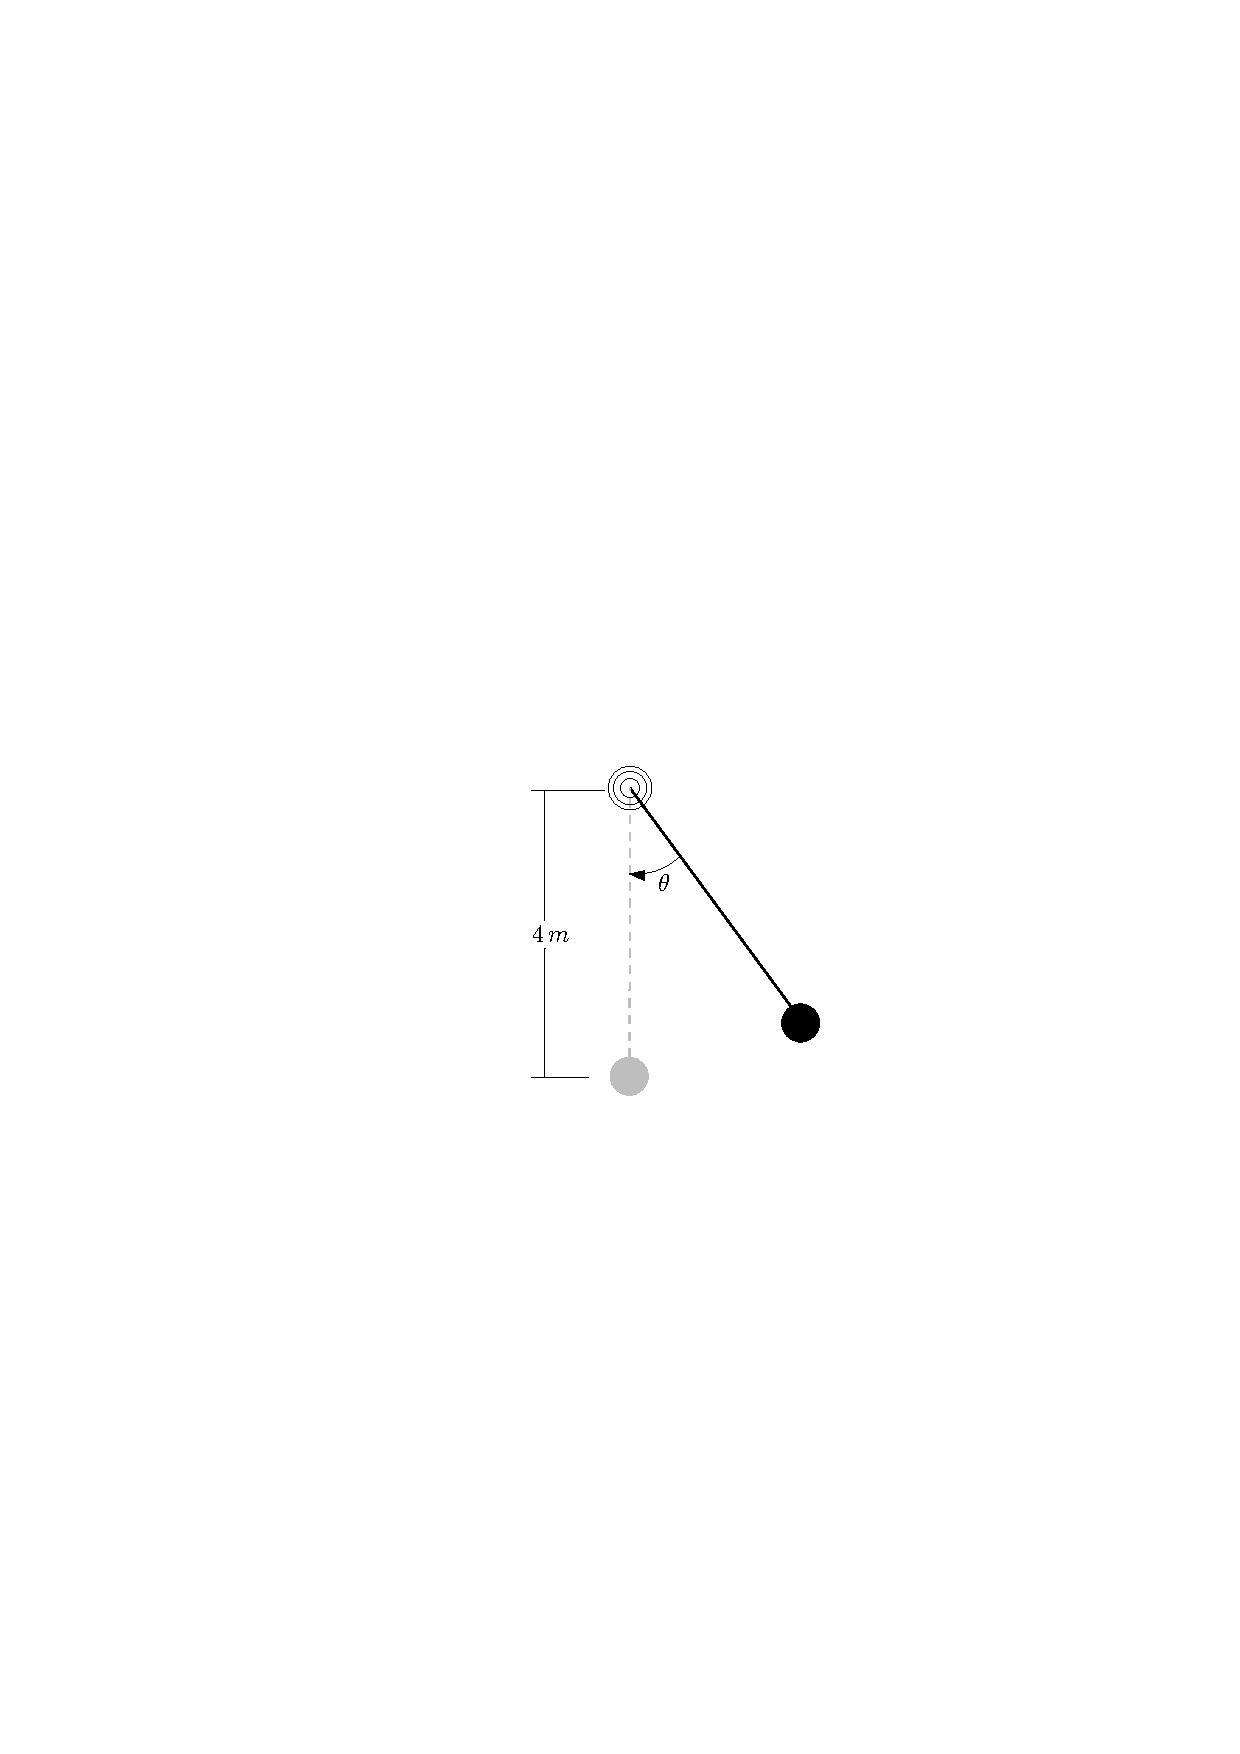
\includegraphics[scale=1.2]{images/draw_12.pdf}
		\end{flushright}
		
		\item Determine a velocidade mínima que deve ser dada à caixa de \SI{2.5}{\kilogram} em $A$ a fim de que ela permaneça em contato com a trajetória circular. Determine também a velocidade da caixa quando ela chega ao ponto $B$
		
		\textbf{Resposta}
		$
		\begin{cases}
		v_{\textit{mín}}=\SI{7.67}{\meter/\second}\\
		v_{B}=\SI{3.86}{\meter/\second}
		\end{cases}
		$
		\vspace{-2cm}
		\begin{flushright}
			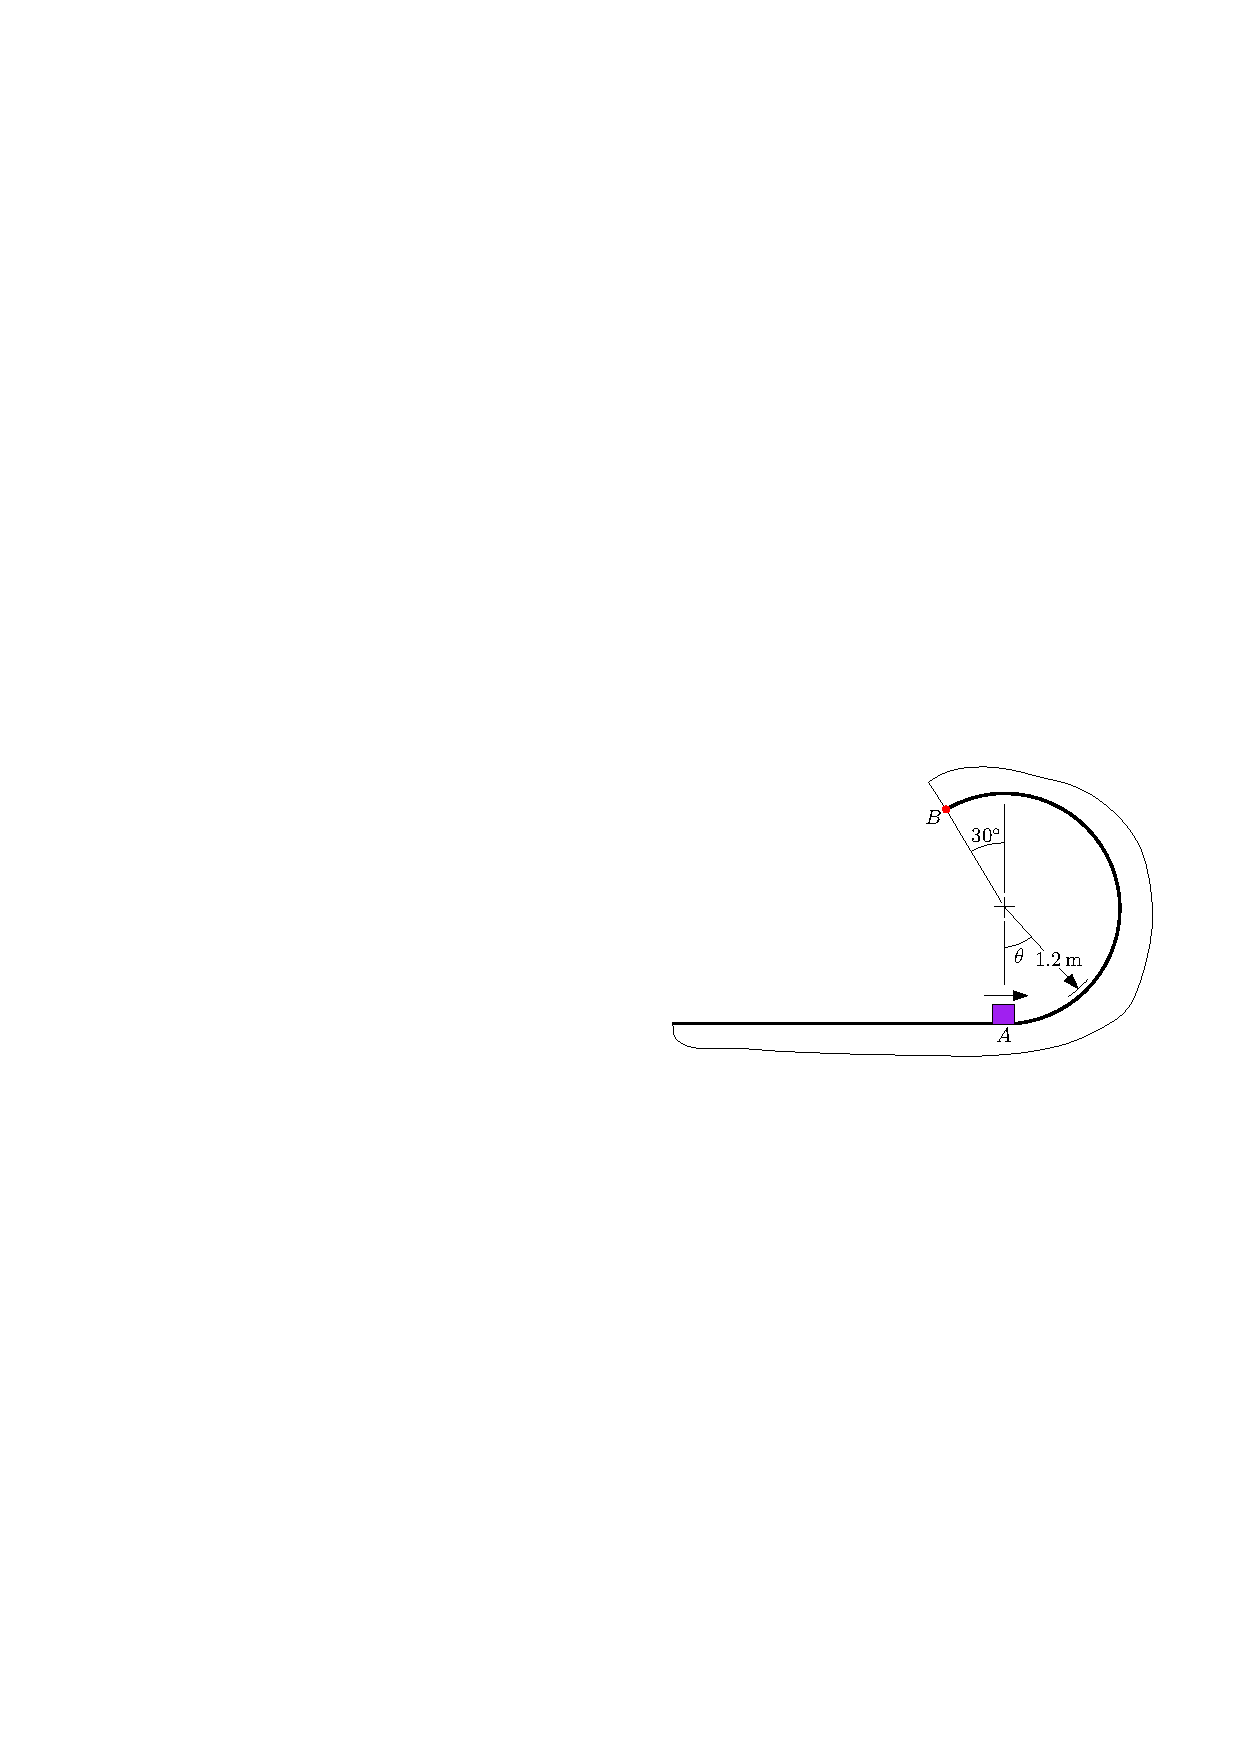
\includegraphics[scale=1.4]{images/draw_6.pdf}
		\end{flushright}
		
		\newpage
		\item Determine a velocidade máxima na qual o carro com massa $m$ pode passar sobre o ponto mais alto $A$ da estrada em curva vertical e ainda manter o contato com a estrada. Se o carro mantém essa velocidade, qual é a reação normal que a estrada exerce sobre o carro quando ele passa pelo ponto mais baixo $B$ na estrada?
		
		\textbf{Resposta}
		$
		\begin{cases}
		v=\sqrt{r\,g}\\
		N=2\,mg
		\end{cases}
		$
		\vspace{-2cm}
		\begin{flushright}
			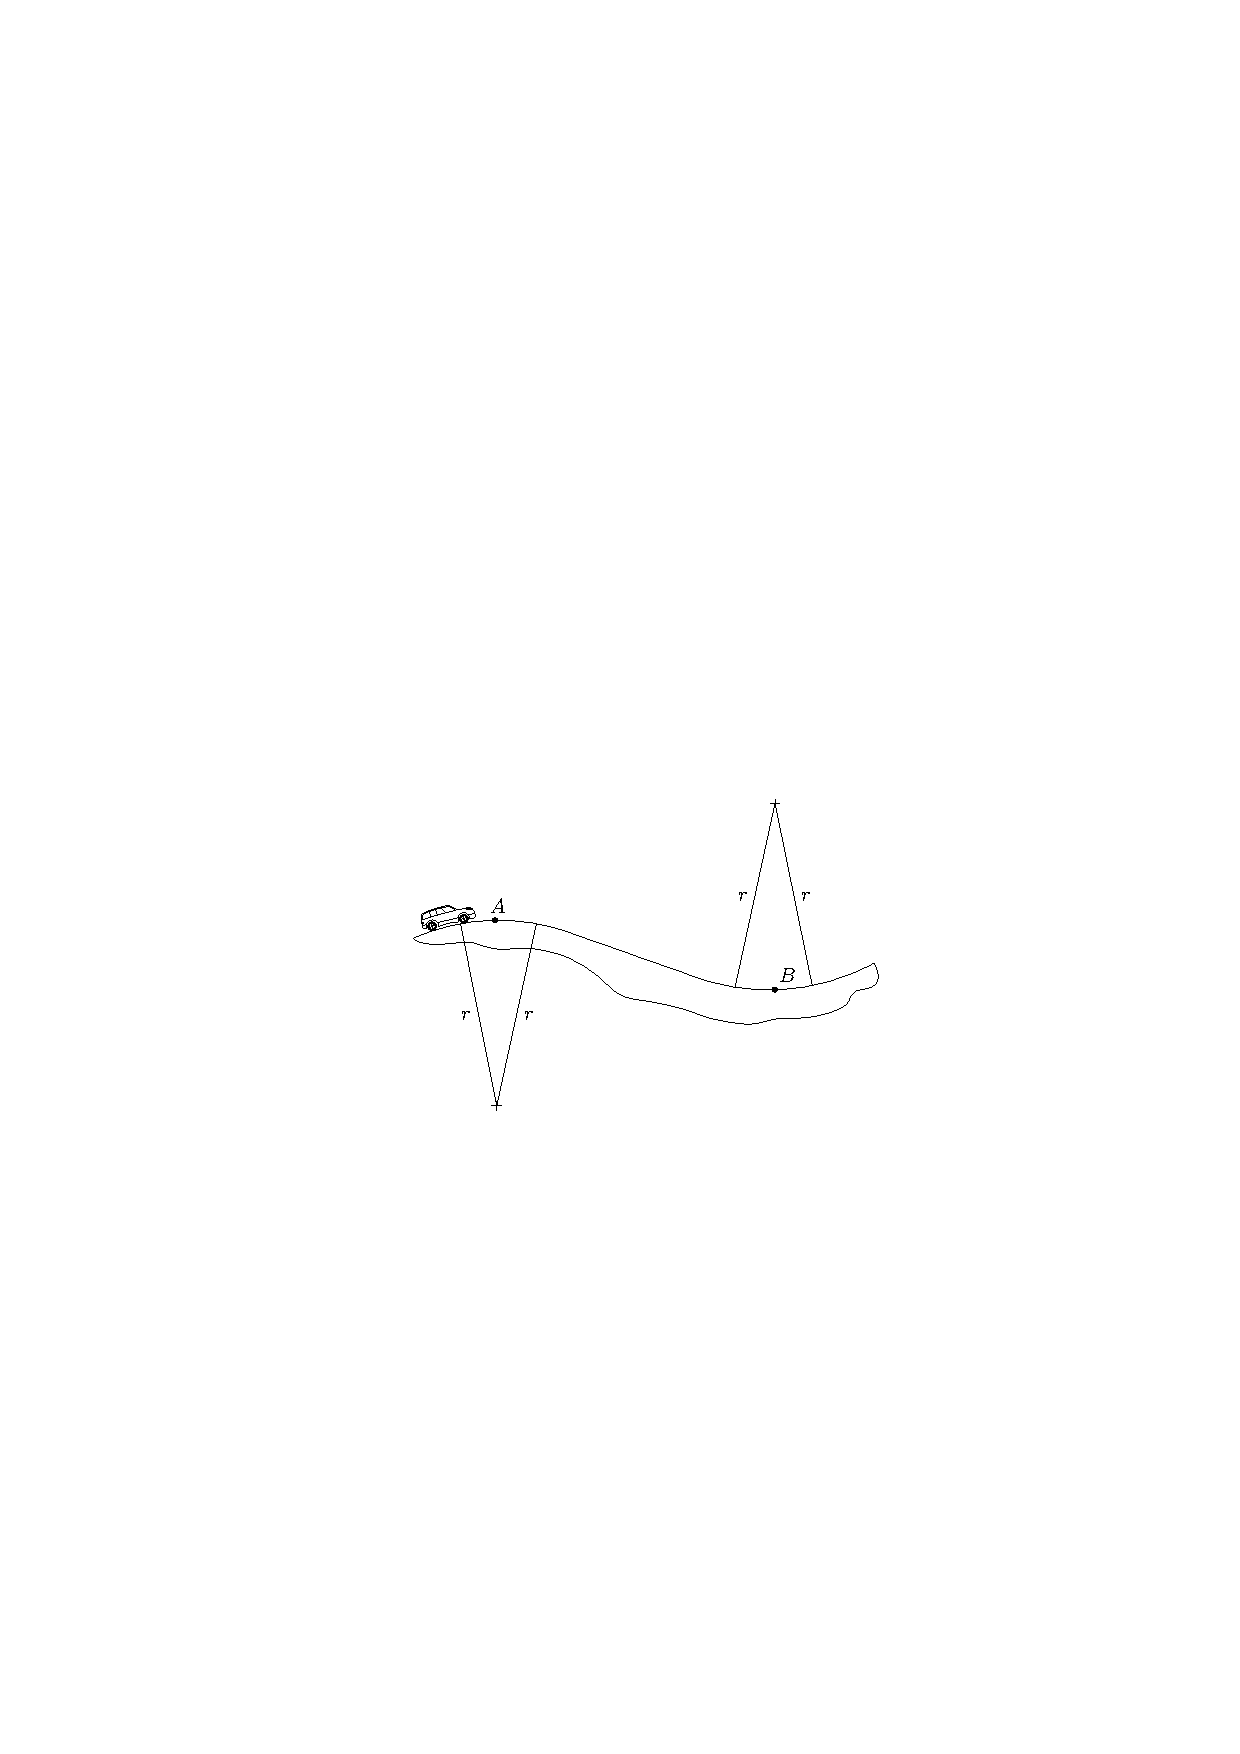
\includegraphics[scale=1.2]{images/draw_10.pdf}
		\end{flushright}
		
		\item A trajetória do movimento de uma partícula de \SI{5}{\kilogram} no plano horizontal é descrita em termos das coordenadas polares como $r= (2\,t+1)$ e $\theta=(0.5\,t^{2}-t)$, onde $t$ é dado em segundos. Determine a intensidade da força resultante atuando sobre a partícula quando $t=\SI{2}{\second}$.
		
		$\textbf{\text{Resposta}}\Rightarrow F=\SI{51.5}{\newton}$
		
		\item O anel $C$ de \SI{0.5}{\kilogram} pode deslizar livremente ao longo da barra lisa $AB$. EM um dado instante, a barra $AB$ está girando com uma  velocidade angular de $\dot{\theta}=\SI{2}{\radian/\second}$ e tem aceleração constante de $\ddot{\theta}=\SI{2}{\radian/\second^{2}}$. Determine a força normal da barra $AB$ e a reação radial da placa na extremidade $B$ sobre o anel neste instante. Despreze a massa da barra e a dimensão do anel.
		
		\textbf{Resposta}
		$
		\begin{cases}
		N_{B}=\SI{1.20}{\newton}\\
		F_{AB}=\SI{0.6}{\newton}
		\end{cases}
		$
		
		\vspace{-2cm}
		\begin{flushright}
			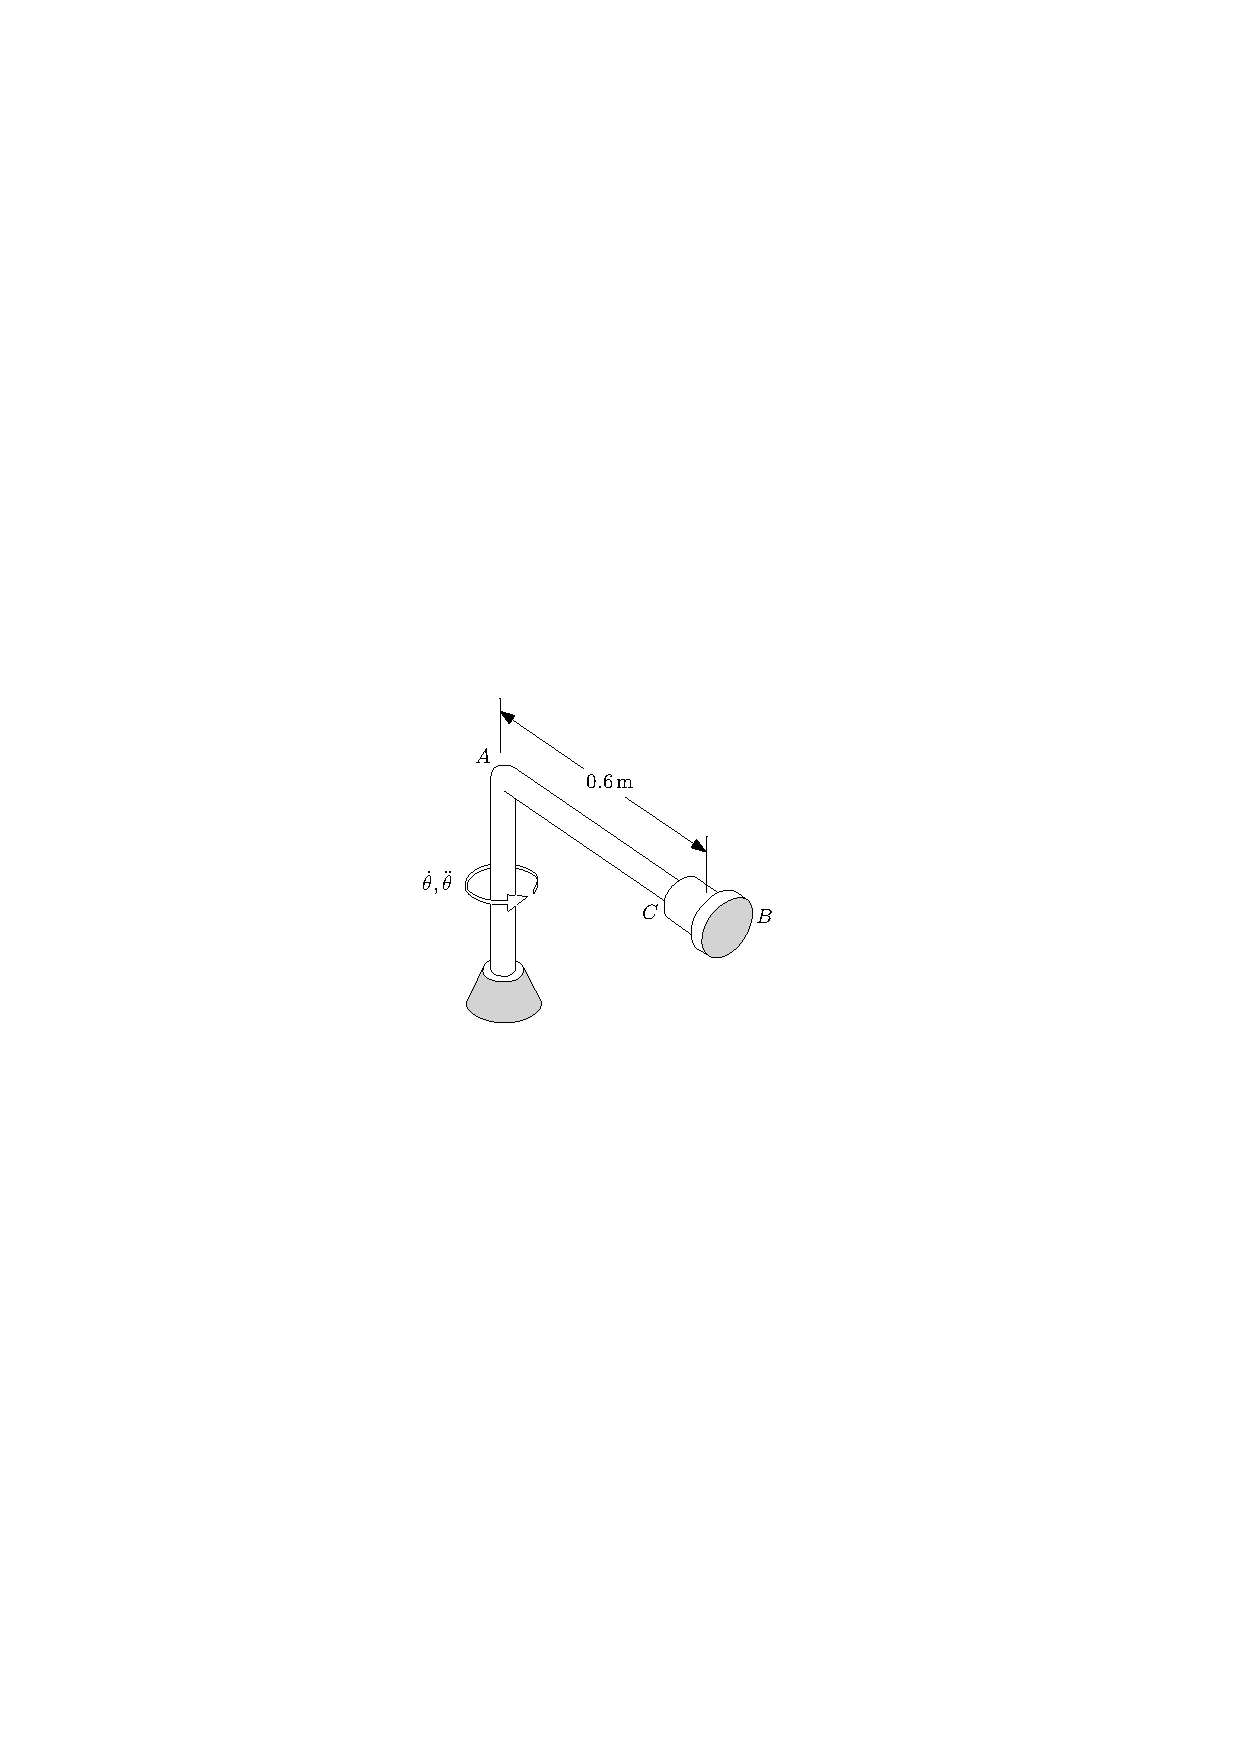
\includegraphics[scale=1.5]{images/draw_7.pdf}
		\end{flushright}
		
		\newpage
		
		\item Utilizando a pressão do ar, a bola de \SI{0.5}{\kilogram} é forçada a se mover por um tubo colocado no plano horizontal com o formato de uma espiral logarítmica. Se a força tangencial exercida sobre a bola devida à pressão do ar é de \SI{6}{\newton}, determine a taxa de aumento na velocidade da bola no instante $\theta=\pi/2$. 
		
		$\textbf{\text{Resposta}}\Rightarrow a_{t}=\SI{12}{\meter/\second}$
		
		\vspace{-1cm}
		\begin{flushright}
			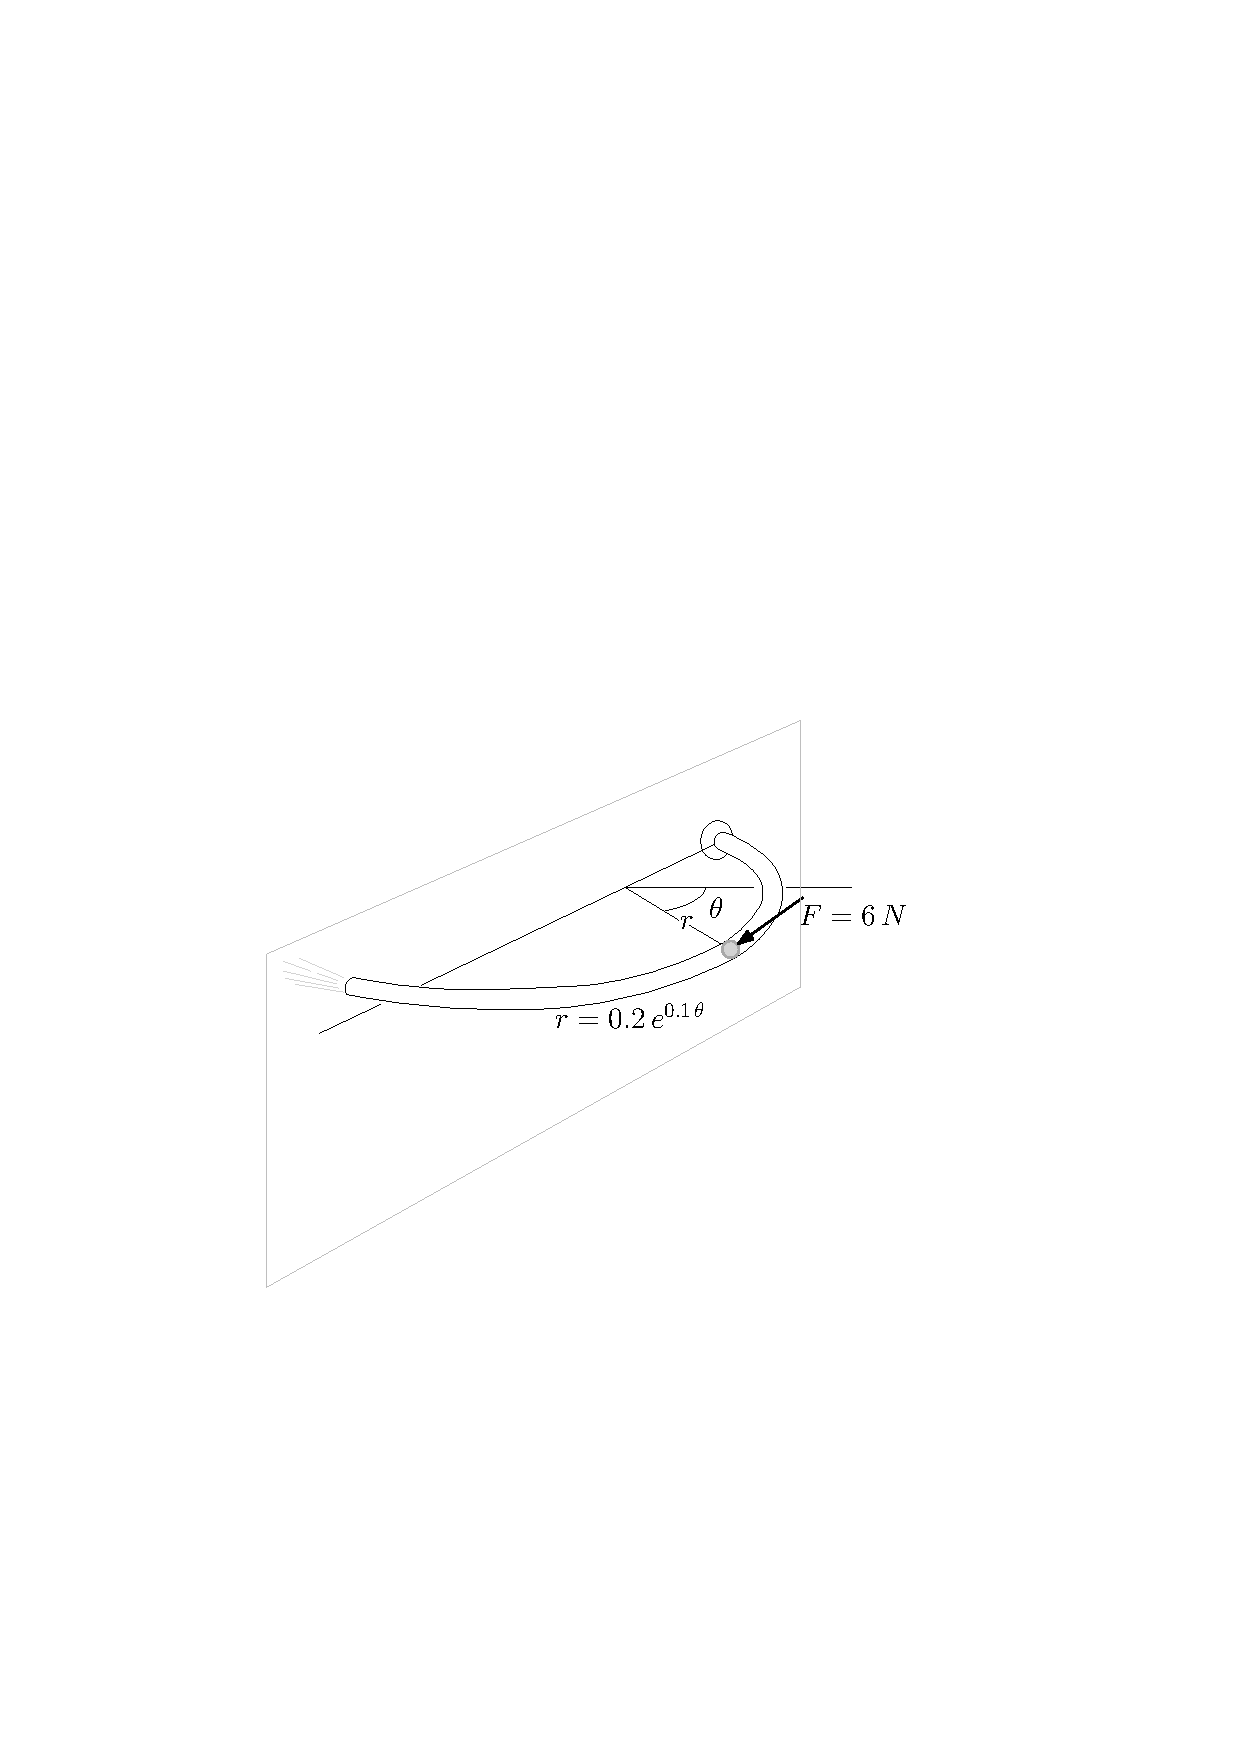
\includegraphics[scale=1]{images/draw_8.pdf}
		\end{flushright}
		
		\item Um brinquedo do parque de diversões gira com uma velocidade angular constante de $\dot{\theta}=\SI{0.8\,}{\radian/\second}$. Se a trajetória do brinquedo é definida por $r=(3\,\sin\theta + 5)\,\SI{}{\meter}$ e $z=(3\,\cos\theta)\,\SI{}{\meter}$, determine as
		componentes da força $r$, $\theta$ e $z$ exercidos pelo assento sobre o garoto de \SI{20}{\kilogram} quando $\theta=\SI{120}{^{\circ}}$.
		
		\textbf{Resposta}
		$
		\begin{cases}
		F_{r}=\SI{-131}{\newton}\\
		F_{\theta}=\SI{-38.4}{\newton}\\
		F_{z}=\SI{215}{\newton}
		\end{cases}
		$
		\vspace{-2.5cm}
		\begin{flushright}
			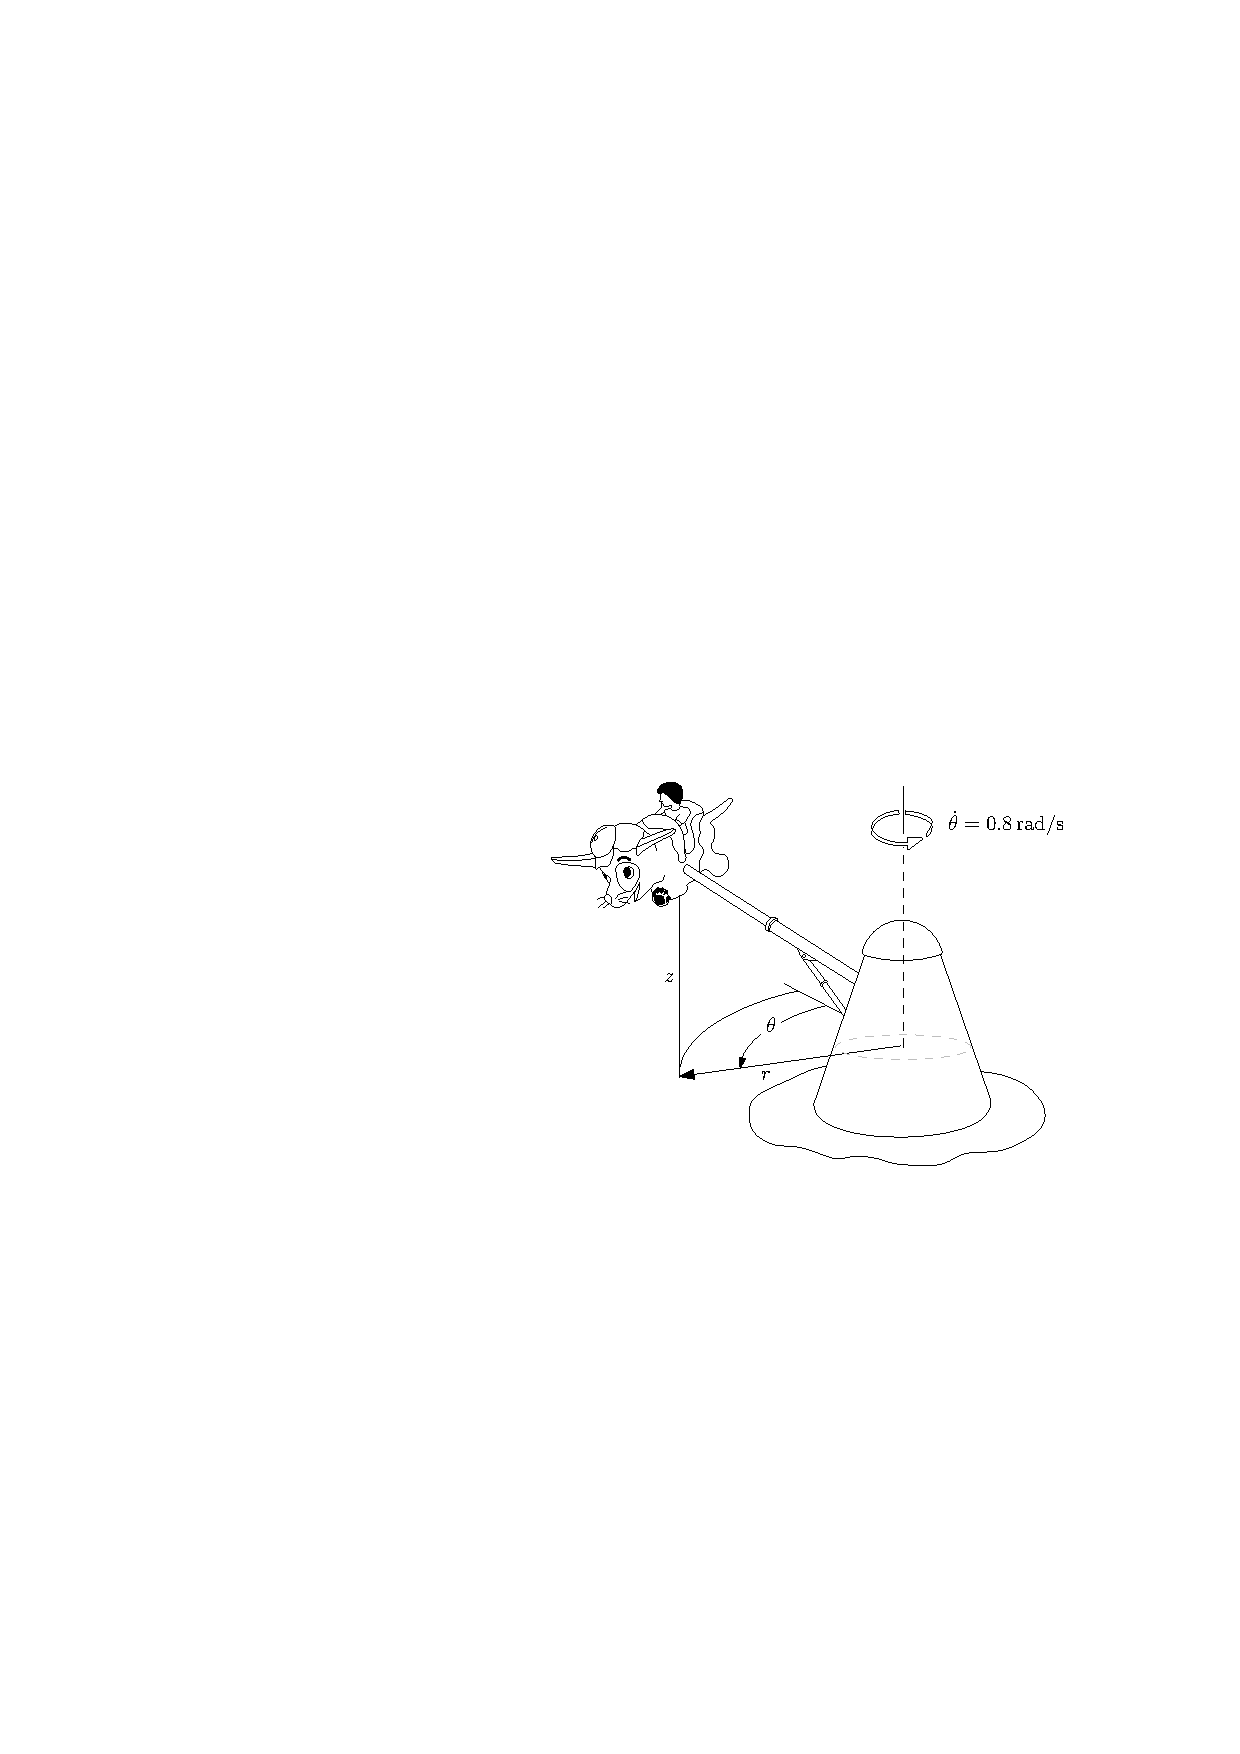
\includegraphics[scale=1.27]{images/draw_13.pdf}
		\end{flushright}
	\end{enumerate}
	
\end{document}